\chapter{Design}\label{Design}

\section{Desired Work-cell}

\begin{figure}[h]
    \centering
    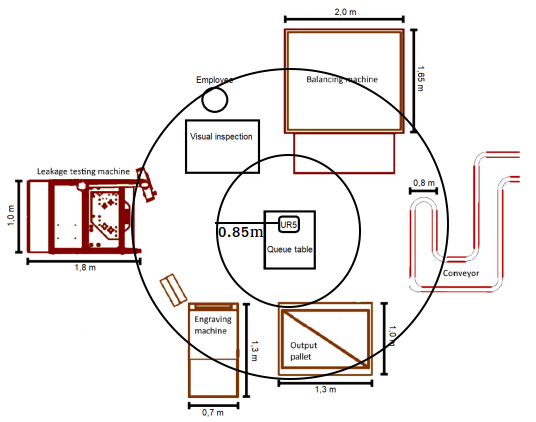
\includegraphics[width=9cm]{Design/Work_cell_3.png}
    \caption{work-cell with measurements and reach}
    \label{fig:workcellMR}
\end{figure}

When looking at \ref{fig:workcellMR}, a systematic work-cell is presented. But the important thing of a work-cell is its flow.\\
Here is some sections about what is needed of the ideal work-cell.

\subsection{Dexterous work-space}

The work-space which a manipulator works within can be described as a radius which the point of the end-effector can reach.\\
The Dexterous work-space is a more intelligent way of the robot to decide which points in arbitrary orientation, can be reached \cite{Dexterous}.\\
The reason that the dexterous work-space is considered a solution to the work-cell, is that the kinematic restrains can be included, so that the trajectories of the manipulator wont freeze or go in lock down.\\


\subsection{Safety}

To keep the production safe and manageable, some of the safety devices are chosen:

\begin{itemize}
    \item Light Curtain
    \item LIDAR
\end{itemize}

The light curtain provides a signal when the curtain is broken, see \ref{SafetyDevices}.\\
This will be used to send a signal to the UR5 to either stop or slow down the production, so a person safely can enter the cell, without getting serious damages.\\

The LIDAR is commonly used in production, see \ref{SafetyDevices}.
This threshold can be used to measure when a person enters the hazardous work area of the UR5.\\
All of the above is a must since the UR5 is carrying a metal rotor with sharp edges, so the person wont be gauged.\\

\subsection{Safety Requirements}

The most important solution for the safety of the work-cell, is the ISO 10218-2:2011, see \ref{ISO2}.\\
When installing a new robot for a production line, some standards is required. These standards of the ISO can present which of the areas needed to be acted upon.\\

\subsection{Placement Sensors}

To ensure the work-flow some intelligent placement sensors must be implemented. Some of the possible solutions are chosen:\\

\begin{itemize}
    \item LIDAR
    \item Photocell sensors
    \item Depth sensing camera
\end{itemize}

The LIDAR is a sensor that gives a 3D view, and can be used for the robot to tell the different object apart, and give an overview of the work-cell, see \ref{ref:PlacementS}.\\
These signals can be used for the cobot to get a better work-flow and also determine objects from each other.\\

The photocell sensors can be used for a quicker work-flow, since it will detect the rotors when they are in the correct place to be picked up, see \ref{ref:PlacementS}.\\

Depth sensing cameras can determine the distance from end-effector to the desired object, see \ref{ref:PlacementS}. This can be used to derive the distance from the certain machine where the rotor has to be placed.\\

\subsection{Conclusion}

When having looked into what an optimal layout for the work-cell could be, with regards to the above sections, it was concluded that it was also necessary to consider the robot manipulators that has to function within this space. 

\section{Desired Robot}\label{IdealRobot}

The ideal robot to have inside the work-cell, is intelligent, fast and can decide the next trajectory without any hesitation. Its size is optimized to fit the given case, to work at the most effective speed possible.\\

\subsection{Desired speed}

The robot has 7 tasks it needs to complete within 26 seconds. This means that the slowest possible speed it has to have per translation to other machines, while delivering the rotor, is 26 divided by 7, which will give the manipulator 3.7142 seconds to carry out the task.\\
Taking the visual inspection in consideration, the number has to be lower when translating from the machines. The person inspecting might need something close to 5 seconds. Taking that into consideration a new formula for the speed of the cobot can be found.\\

\begin{equation}
    26 = 5 + 6 \times b \Rightarrow b = \frac{21}{6}\\
\end{equation}

\begin{equation}
    b = \frac{21}{6} \Rightarrow b = \frac{7}{2}\\
\end{equation}

\begin{equation}
    b = \frac{7}{2} \Leftrightarrow  b = 3.5 sec\\
\end{equation}

5 seconds in one station means that the other stations needs to be cut down with 0.2 seconds each.\\
So the optimal speed for translations would be 3.5 seconds.\\

\subsection{Desired reach}

The manipulator must be able to reach all pick and place points, without having to move its base. Given the work-cell design, this means the robot will need a reach of 2 meters. \\
\begin{figure}[H]
    \centering
    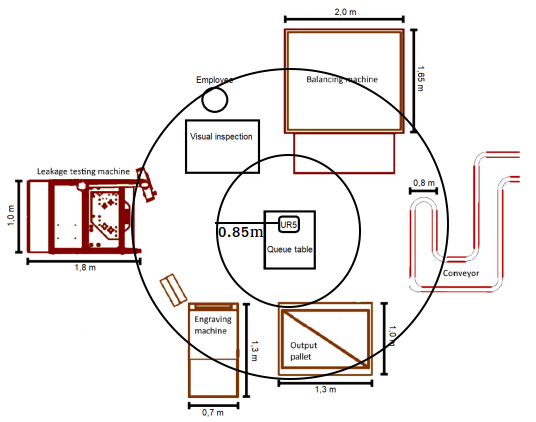
\includegraphics[width=8cm]{Design/Work_cell_3.png}
    \caption{Work-cell with measurements and reach}
    \label{fig:workcell}
\end{figure}

This desired reach could also be accomplished by changing the setup to use 2 manipulators, see figure \ref{fig:workscell2arms}. By doing it this way, the 2 robots would only need one place where their reach overlap, so they can both pick and place the rotors on a buffer table. This would also require additional programming, which should prevent the two robots from hitting each other.\\

\begin{figure}[H]
    \centering
    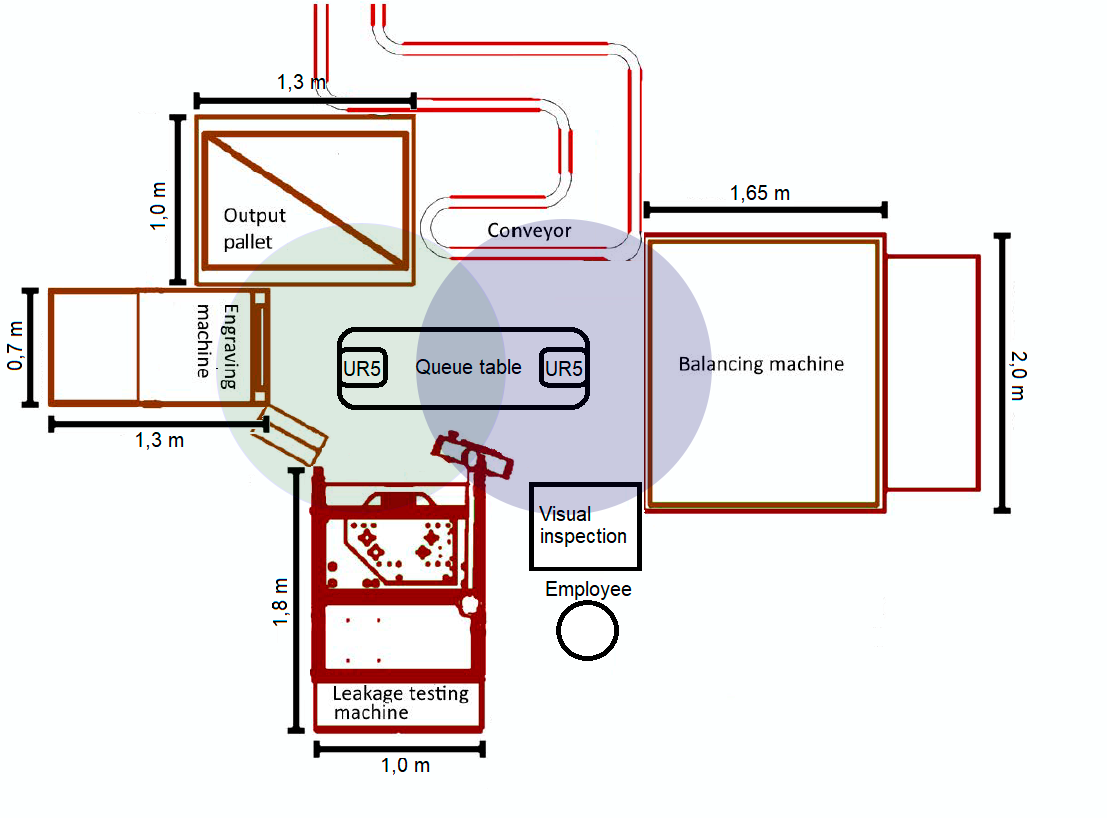
\includegraphics[width=.5\textwidth]{Design/Work_cell_8.PNG}
    \caption{Work-cell design with 2 robots}
    \label{fig:workscell2arms}
\end{figure}

\begin{figure}[H]
  \centering
  \begin{minipage}[b]{0.45\textwidth}
    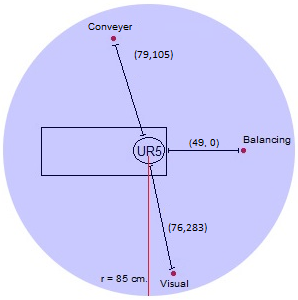
\includegraphics[width=\textwidth]{Design/workcell_1_polar.png}
    \label{fig:position}
  \end{minipage}
  \hfill
  \begin{minipage}[b]{0.45\textwidth}
    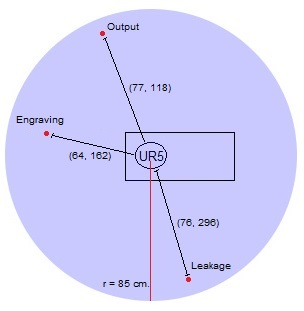
\includegraphics[width=\textwidth]{Design/polar.jpg}  
    \label{fig:velocity}
  \end{minipage}
  {Work-cell first and second part ,with polar coordinates and reach to suited the reach of the UR 5.}
\end{figure}
%Flowchart 1:
\begin{tikzpicture}[node distance=2cm]

%Primary nodes:
\node (start) [startstop] {Rotor arrives on conveyer/queue table};
\node (dec1) [decision, below of=start, yshift=-2.5cm] {Has this rotor been balance tested?};
\node (dec2) [decision, right of=dec1, xshift=3.2cm] {Is the balancing
machine empty?};
\node (pro1) [process, right of=dec2, xshift=3.1cm] {Move the rotor to balancing machine};
\node (out1) [io, below of=pro1, yshift=-3cm] {Balancing complete};
\node (dec3) [decision, below of=dec1, yshift=-6cm] {Has this rotor been visually inspected?};
\node (dec4) [decision, right of=dec3, xshift=3.2cm] {Is visual inspection available?};
\node (pro2) [process, right of=dec4, xshift=3.1cm] {Move the rotor to visual inspection};
\node (out2) [io, below of=pro2, yshift=-3cm] {Visual inspection complete};
\node (stop) [startstop, below of=dec3, yshift=-5cm] {Move rotor to queue table};

%Primary arrows:
\draw [arrow] (start) -- (dec1);
\draw [arrow] (dec1) -- node[anchor=south] {no} (dec2);
\draw [arrow] (dec1) -- node[anchor=west] {yes} (dec3);
\draw [arrow] (dec2) -- node[anchor=south] {yes} (pro1);
\draw [arrow] (pro1) -- (out1);
\draw [arrow] (dec3) -- node[anchor=south] {no} (dec4);
\draw [arrow] (dec3) -- node[anchor=west]  {yes} (stop);
\draw [arrow] (dec4) -- node[anchor=south] {yes} (pro2);
\draw [arrow] (pro2) -- (out2);

%dec2, dec4 -> start:
\node (gui1) [Guidebox, left of=pro1, xshift=-11cm] {};
\node (gui2) [Guidebox, below of=gui1, yshift=-0.85cm] {};
\node (gui6) [Guidebox, left of=pro2, xshift=-11cm] {};
\node (gui7) [Guidebox, below of=gui6, yshift=-0.85cm] {};

%Below dec2:
\node (gui3) [Guidebox, right of=gui2, xshift=5.9cm] {};
\node (gui4) [Guidebox, below of=gui3, yshift=1.9cm] {};
\node (gui5) [Guidebox, right of=gui3, xshift=-1.9cm] {};
\draw [arrow] (dec2) -- node[anchor=west] {no} (gui4);
\draw [arrow] (gui5) -- (gui2);

%Below dec4:
\node (gui8) [Guidebox, right of=gui7, xshift=5.9cm] {};
\node (gui9) [Guidebox, below of=gui8, yshift=1.9cm] {};
\node (gui10) [Guidebox, right of=gui8, xshift=-1.9cm] {};
\draw [arrow] (dec4) -- node[anchor=west] {no} (gui9);

%Line to start:
\node (gui11) [Guidebox, above of=gui1, yshift=2.55cm] {};
\node (gui12) [Guidebox, above of=gui11, yshift=-1.9cm] {};
\node (gui13) [Guidebox, left of=gui11, xshift=1.9cm] {};
\node (gui16) [Guidebox, below of=gui7, yshift=1.9cm] {};
\node (gui17) [Guidebox, left of=gui7, xshift=1.9cm] {};
\draw [arrow] (gui10) -- (gui17);
\draw [arrow] (gui16) -- (gui12);
\draw [arrow] (gui13) -- (start);

%out1, out2 -> dec3, stop:
\node (gui14) [Guidebox, above of=dec3, yshift=1cm] {};
\draw [arrow] (out1) -- (gui14);
\node (gui15) [Guidebox, above of=stop, yshift=-0cm] {};
\draw [arrow] (out2) -- (gui15);

%Caption:
\node (cap1) [Caption, below of=dec4, yshift=-7cm] {This flowchart shows the process performed by the first UR5 in the work-cell.};

\label{fig:first-part}
\end{tikzpicture}


%Flowchart 2:
\begin{tikzpicture}[node distance=2cm]

%Primary nodes:
\node (start) [startstop] {Rotor arrives on queue-table};
\node (dec1) [decision, below of=start, yshift=-2.5cm] {Has this rotor been leak tested?};
\node (dec2) [decision, right of=dec1, xshift=3.2cm] {Is the leak testing
machine empty?};
\node (pro1) [process, right of=dec2, xshift=3.1cm] {Move the rotor to leak testing machine};
\node (out1) [io, below of=pro1, yshift=-3cm] {Leak testing complete};
\node (dec3) [decision, below of=dec1, yshift=-6cm] {Has this rotor been engraved?};
\node (dec4) [decision, right of=dec3, xshift=3.2cm] {Is the engraving
machine empty?};
\node (pro2) [process, right of=dec4, xshift=3.1cm] {Move the rotor to engraving machine};
\node (out2) [io, below of=pro2, yshift=-3cm] {Engraving complete};
\node (stop) [startstop, below of=dec3, yshift=-5cm] {Move rotor to output pallet};

%Primary arrows:
\draw [arrow] (start) -- (dec1);
\draw [arrow] (dec1) -- node[anchor=south] {no} (dec2);
\draw [arrow] (dec1) -- node[anchor=west] {yes} (dec3);
\draw [arrow] (dec2) -- node[anchor=south] {yes} (pro1);
\draw [arrow] (pro1) -- (out1);
\draw [arrow] (dec3) -- node[anchor=south] {no} (dec4);
\draw [arrow] (dec3) -- node[anchor=west]  {yes} (stop);
\draw [arrow] (dec4) -- node[anchor=south] {yes} (pro2);
\draw [arrow] (pro2) -- (out2);

%dec2, dec4 -> start:
\node (gui1) [Guidebox, left of=pro1, xshift=-11cm] {};
\node (gui2) [Guidebox, below of=gui1, yshift=-0.85cm] {};
\node (gui6) [Guidebox, left of=pro2, xshift=-11cm] {};
\node (gui7) [Guidebox, below of=gui6, yshift=-0.85cm] {};

%Below dec2:
\node (gui3) [Guidebox, right of=gui2, xshift=5.9cm] {};
\node (gui4) [Guidebox, below of=gui3, yshift=1.9cm] {};
\node (gui5) [Guidebox, right of=gui3, xshift=-1.9cm] {};
\draw [arrow] (dec2) -- node[anchor=west] {no} (gui4);
\draw [arrow] (gui5) -- (gui2);

%Below dec4:
\node (gui8) [Guidebox, right of=gui7, xshift=5.9cm] {};
\node (gui9) [Guidebox, below of=gui8, yshift=1.9cm] {};
\node (gui10) [Guidebox, right of=gui8, xshift=-1.9cm] {};
\draw [arrow] (dec4) -- node[anchor=west] {no} (gui9);

%Line to start:
\node (gui11) [Guidebox, above of=gui1, yshift=2.55cm] {};
\node (gui12) [Guidebox, above of=gui11, yshift=-1.9cm] {};
\node (gui13) [Guidebox, left of=gui11, xshift=1.9cm] {};
\node (gui16) [Guidebox, below of=gui7, yshift=1.9cm] {};
\node (gui17) [Guidebox, left of=gui7, xshift=1.9cm] {};
\draw [arrow] (gui10) -- (gui17);
\draw [arrow] (gui16) -- (gui12);
\draw [arrow] (gui13) -- (start);

%out1, out2 -> dec3, stop:
\node (gui14) [Guidebox, above of=dec3, yshift=1cm] {};
\draw [arrow] (out1) -- (gui14);
\node (gui15) [Guidebox, above of=stop, yshift=-0cm] {};
\draw [arrow] (out2) -- (gui15);

%Caption:
\node (cap1) [Caption, below of=dec4, yshift=-7cm] {This flowchart shows the process performed by the second UR5 in the work-cell.};

\end{tikzpicture}






\subsection{Desired sensors}

The robot should be able to identify humans, and collisions must be risk free, and not disrupt the work-flow. Optimally, the robot should also be able to identify what object it is holding, and if it is damaged or not. Additionally, the robot must be able to place the rotors correctly in the machines, using a depth sensing camera. \ref{depthcam}\\
The robot should be able to register whether or not it has picked up a rotor. This can be done by using a pressure sensor.\\ 

\subsection{Max payload}
The robot manipulator must be able to lift the combined weight of the L40 rotor, aswell as the end-effector tool meant to lift and move the rotor. For this reason, the combined weight of the end-effector tool and the L40 rotor can not exceed a total weight of 5 Kg.\\

%\ref{workscell2arms}. this ref is not linking to anything??
%The robot must be able to lift the L40 rotor given in the case, which weighs 645 grams. The end-effector must also be able to grab it, without the risk of dropping it. The rotor is 190mm long, and 90mm wide at its widest point. The manipulator must also be able to support the[width=8cm] weight when the arm is fully stretc\ref{workscell2arms}

\subsection{Conclusion}

From this chapter several specifications can be derived, which is required to setup a robot manipulator, these data and considerations will thus be used for the next section, which will describe these requirements.


\section{Denavit-Hartenberg}

In order to enable the UR5 on the flexible workstation to locate itself and its surroundings within a space, the DH (Denavit-Hartenberg) method is used.\\ 
The DH method can be used to compute every frame into parameters.\\
These descriptions of the system can be used to translate every point and every movement of the robotic manipulator, with the help of forward kinematic.\\
Initially the start is to locate all of the coordinate systems, as seen in \ref{table:1}.\\ 


\begin{itemize}
    \item ${a_{i-1}}$= The distance from ${Z_{i-1}}$ to ${Z_{i}}$ measured along ${X_{i-1}}$
    \item ${\alpha_{i-1}}$ = The angel between ${Z_{i-1}}$ to ${Z_{i}}$ measured about ${X_{i-1}}$
    \item ${d_{i}}$ = The distance from ${X_{i-1}}$ to ${X_{i}}$ measured along ${Z_{i}}$
    \item ${\theta_{i-1}}$ = The angel between ${X_{i-1}}$ to ${X_{i}}$ measured about ${Z_{i}}$
\end{itemize}



Then the angles and the distance from each coordinate system is computed and set in to a table as seen in \ref{fig:DH-Table}.

\begin{figure}[h!]
    \centering
    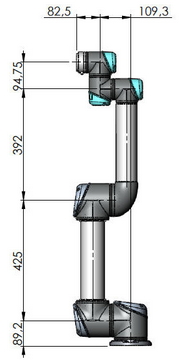
\includegraphics[scale=0.79]{Design/UR5measure.png}
    \caption{UR5 to describing DH-parameters \cite{DH}} 
    \label{fig:DH-Table} 
\end{figure}

%\begin{table}[h!]
%\centering
%\begin{tabular}{||c c c c c||} 
% \hline
% i & \alpha_{i-1} & a_{i-1} & d_{i} & \theta_{i} \\ [0.5ex] 
% \hline\hline
% 1 & 0 & 0  & 0     & \theta_{1} \\ 
% 2 & 0 & l_{1} & 0 & \theta_{2} \\
% 3 & 0 & l_{2} & 0 & \theta_{3} \\[1ex]
% \hline
%\end{tabular}
%\caption{DH-Table}
%\label{table:DH-table}
%\end{table}

As seen in \ref{fig:DH-Table},the coordinate systems is used to trace every step of each axis.\\
Starting from left to right at the top of the table, the $\alpha-1$ is used to compute the differences of the angles between $Z_{i}$ and $Z_{i-1}$, which is 0, due to the fact that they keep the same angle from $Z_{i}$  to $Z_{i-1}$.\\
It can also be seen from the table that the distance between $Z_{i}$ and $Z_{i-1}$ is Length2, since they are parallel to each other.\\ 
The distance between $X_{i-1}$ and $X_i$ is 0 since they cross each other on the perpendicular line, which means that in that point the new coordinate system should be placed.\\

\begin{table}[h!]
\centering
\begin{tabular}{||c c c c c||} 
 \hline
 i & $\alpha_{i-1}$ & $a_{i-1}$ & $d_{i}$ & $\theta_{i}$ \\ [0.5ex] 
 \hline 
 \hline
 1 & 0 & 0 & 89.2 & $\theta_{1}$ \\ 
 2 & 90 & 0 & 0 & $\theta_{2}$ \\
 3 & 0 & 425 & 0 & $\theta_{3}$ \\
 4 & 0 & 392 & 109.3 & $\theta_{4}$ \\
 5 & -90 & 0 & 94.75 & $\theta_{5}$ \\ 
 6 & 90 & 0 & 82.5 & $\theta_{6}$ \\[1ex] 
 \hline
\end{tabular}
\caption{DH-parameters for the UR5, using \cite{DHPar} as measurement.}
\label{table:1}
\end{table}

\section{Forward Kinematics}
Forward kinematics can be used for calculating the position and orientation of the end-effector of a robotic manipulator. This can be done by using the matrices describing the position and orientation of each of the joints for the specific robotic manipulator, and the following formula: \\

\begin{equation}
    _N^0 T\; =\ _1^0T\  _2^1T\  _3^2T\  _4^3T\  .........\  _N^{N-1}T\\
\end{equation} \\

This is the formula used for calculating the end-effector of a robotic manipulator. \\

Now, the required transformation matrices can simply be inserted into the formula, and the matrix describing the position of the end-effector can be calculated. \\

Below are the general transformation matrices used in this method; from the base of the robotic manipulator to the sixth joint. These can be multiplied together to find \(_6^BT\) for the UR5: 

\begin{equation}
\centering
_i^{i-1}T = \begin{bmatrix} Cos(\theta_i) & -Sin(\theta_i) & 0 & a_{i-1}\\
Sin(\theta_i)*Cos(\alpha_{i-1}) & Cos(\theta_i)*Cos(\alpha_{i-1}) & -Sin(\alpha_{i-1}) & -Sin(\alpha_{i-1})*d_i\\
Sin(\theta_i)*Sin(\alpha_{i-1})& Cos(\theta_i)*Sin(\alpha_{i-1}) & Cos(\alpha_{i-1}) & Cos(\alpha_{i-1})*d_i \\
0 & 0 & 0 & 1\\ \end{bmatrix}
    \caption{Caption}
    \label{fig:my_label}
\end{equation}
\\


\begin{equation}
\centering
_0^BT = \begin{bmatrix} 1&0&0&0\\0&1&0&0\\0&0&1&0\\ 0&0&0&1\end{bmatrix}
    \caption{Caption}
    \label{fig:tb0}
\end{equation}

\begin{equation}
\centering
_1^0T = \begin{bmatrix} Cos(\theta_1)&-Sin(\theta_1)&0&0\\Sin(\theta_1) & Cos(\theta_1)&0&0\\0&0&1& d_1\\0&0&0&1 \end{bmatrix}
    \caption{Caption}
    \label{fig:t01}
\end{equation}

\begin{equation}
\centering
_2^1T = \begin{bmatrix} Cos(\theta_2)&-Sin(\theta_2)&0&0\\
0&0&-1&0\\Sin(\theta_2)& Cos(\theta_2)&0&0\\0&0&0&1\end{bmatrix}
    \caption{Caption}
    \label{fig:t12}
\end{equation}

\begin{equation}
\centering
_3^2T = \begin{bmatrix} Cos(\theta_3)&-Sin(\theta_3)&0&a_2\\
Sin(\theta_3)&Cos(\theta_3)&0&0\\0&0&1&0\\0&0&0&1\end{bmatrix}
    \caption{Caption}
    \label{fig:t23}
\end{equation}
\begin{equation}
\centering
_4^3T = \begin{bmatrix} Cos(\theta__4)&-Sin(\theta_4)&0&a__3\\
Sin(\theta_4)&Cos(\theta_4)&0&0\\0&0&1& d_4\\0&0&0&1\end{bmatrix}
    \caption{Caption}
    \label{fig:t34}
\end{equation}

\begin{equation}
\centering
_5^4T = \begin{bmatrix} Cos(\theta_5)&-Sin(\theta_5)&0&0\\
0&0&1&d_5\\-Sin(\theta_5)&-Cos(\theta_5)&0&0\\0&0&0&1\end{bmatrix}
    \caption{Caption}
    \label{fig:t45}
\end{equation}

\begin{equation}
\centering
_6^5T = \begin{bmatrix} Cos(\theta_6)&-Sin(\theta_6)&0&0\\https://www.sharelatex.com/project/5a829b040d7aa54a74a65ba0
0&0&-1&-d_6\\Sin(\theta_6)&Cos(\theta_6)&0&0\\0&0&0&1\end{bmatrix}
    \caption{Caption}
    \label{fig:t56}
\end{equation}

 \\\


The main idea is, given the joint angles as input, you would be able to get the coordinates for the end-effector as output. So the position can be calculated from specific set values, and used for simulations.\\

Kinematics can be used to form an internal picture in a cartesian space  of the robot movements, and help understanding and explaining it. 

This is useful when working with not only manipulators, but also animations in movies and video games, or any other movement where multiple joints are used. 



\section{Inverse Kinematics}
Inverse kinematics is used to compute the joint angles from a given position and orientation of an object\cite{JohnC}. The inverse kinematic can be set up from two aspects, one is the geometric way and the other is an algebraic solution, the one the team is using is the algebraic solution where the inverse kinematics is set up in MATLAB, a math computer program, where it makes it possible to be used later in computing the trajectory of the manipulator.\\




\section{Conclusion} 

Describing a robot with forward kinematics and Denavit-Hartenberg parameters is used to locate the different joints and the tool in 3D-space, so the robot can be manipulated and used for various tasks.\\
Looking at Denavit-Hartenberg, the advantage of this method is to simplify the different axis in a matrix, so the operator and the robot can identify where the different coordinate systems is located.\\
Forward kinematics is the starting point of selecting the DH-parameters, when we know the point $Z_{1-1}$ and $Z_1$ we can then locate every axis in the desired robot. Hereby conclude to DH-parameters and include them into MATLAB while visualizing the robot and locate the robot so the tasks can be performed.\\











